\documentclass[tikz,border=6pt]{standalone}
\usepackage{xcolor}
\usetikzlibrary{arrows.meta,positioning}

\definecolor{blockblue}{HTML}{4A90D9}
\definecolor{linegray}{HTML}{333333}

\begin{document}
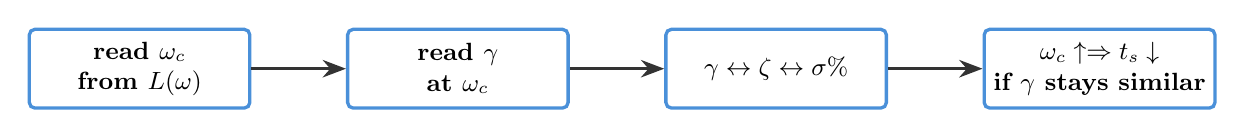
\begin{tikzpicture}[
  >=Stealth,
  line width=1.2pt,
  stage/.style={rectangle, draw=blockblue, rounded corners=2pt, minimum width=2.8cm, minimum height=1.0cm, align=center, font=\small\bfseries},
  flow/.style={->, draw=linegray, line width=1.2pt}
]
  \node[stage] (s1) at (0,0) {read $\omega_c$\\from $L(\omega)$};
  \node[stage, right=1.2cm of s1] (s2) {read $\gamma$\\at $\omega_c$};
  \node[stage, right=1.2cm of s2] (s3) {$\gamma \leftrightarrow \zeta \leftrightarrow \sigma\%$};
  \node[stage, right=1.2cm of s3] (s4) {$\omega_c \uparrow \Rightarrow t_s \downarrow$\\if $\gamma$ stays similar};
  \draw[flow] (s1) -- (s2);
  \draw[flow] (s2) -- (s3);
  \draw[flow] (s3) -- (s4);
\end{tikzpicture}
\end{document}
